\documentclass[a4paper,11pt,twoside]{article}		% The default is NOT A4!

\usepackage[margin=1.75cm]{geometry}		% I almost always use this package to reduce the massive default margins
\usepackage[square,numbers]{natbib}		% The bibstyle I like uses Name(Year) referencing by default. This forces it to use [#] instead.
\usepackage{amsmath}						% amsmath adds various operators and symbols, but most importantly includes the 'align' display math environment
\usepackage{amssymb}						% ...adds extra maths symbols. Couldn't honestly tell you whether I use this all the time or not at all -- it's just always there.
\usepackage{graphicx}					% Required to include graphics.
\usepackage{hyperref}					% Adds hyperlinks to the table of contents, references, cross-references, and urls given the \url{} tag, when output is a pdf. MUST BE LOADED BEFORE cleveref! 
\usepackage{cleveref}					% Introduces the \cref{} command for cross referencing -- automatically adds the right label to a reference. Otherwise prepare for lots of 'Figure~\ref{}'.
\usepackage[section]{placeins}			% Allows a bit more control of graphic placement by the inclusion of the \FloatBarrier command. The 'section' option does this automatically at sections.
\usepackage{aurical}						% This and fontenc are just here to facilitate that awful subtitle font I've used. Sorrynotsorry.
\usepackage[T1]{fontenc}

\author{Oliver Thomson Brown}
\title{\textbf{Example \LaTeX\ Document} \\ {\Fontamici Demonstrating A Selection Of Features Most Arbitrary}}
\date{}

\begin{document}

\maketitle

\tableofcontents

\section{General Text}
\label{sec:1}

There are a few things relating to simply writing text in \LaTeX\ that probably bear mentioning. First of all quotes -- simply using the single quote mark key on your keyboard leads to 'this'. To get an opening quote mark you actually need to use the backtick key, which is just left of the `1' key on a UK keyboard. Additionally, one should never use the double quote key, as "this" happens. The proper procedure is two backticks to open, and two single quote marks to close -- ``wonderful''. What if you need to use both? Then you need to use \verb:\,: to separate them which typesets a thin space. ``It must be admitted that certain things in \LaTeX\ are quite `tiresome'\,''.

Moving on to dashes -- did you know there are actually three?! The one I've been using so far, the humble em dash `--' is typeset by \verb:--: and is a long pause, useful for separating sentences and clauses. Then there's the hyphen, used to combine words like `Heriot-Watt', which is typeset by \verb:-:. Finally there is the en dash `---', which apparently means `through' as in `pages 11---15', and I don't think I have ever bothered to use it. So there you go.

The final thing I can think to mention here is paragraphs. Compiling the document you will see that each of these paragraphs after the first is tab indented, though inspection of the source will show you that all the text is left-aligned with a blank line between. In general \LaTeX\ ignores whitespace, so if I introduce a line-break and tab indent in the source code here:
	\LaTeX\ just ignores it.

On the other hand if I leave a blank line between the previous sentence and this one I am asking \LaTeX\ to treat this as a separate paragraph, and essentially requesting that it do `the right thing'. One can request a line-break using a double backslash.\\ Like so. 

\section{Mathematics}
\label{sec:2}

As mentioned in the presentation there are two main `math(s) modes', inline and display. Inline is accessed with the delimiters \verb:\(: and \verb:\):, and produces unlabelled inline equations like \(M = USV^{\dagger}\). On the other hand display mode is invoked by beginning an equation environment with \verb:\begin{equation}:, and produces separate labelled equations like,
\begin{equation}
\hat{H} = \sum_{i}^{N} \left[ \Delta_{01}\hat{a}_{i}^{\dagger}\hat{a}_{i} + \left(\frac{\Delta_{02}}{2} - \Delta_{01}\right)\hat{a}_{i}^{\dagger}\hat{a}_{i}^{\dagger}\hat{a}_{i}\hat{a}_{i} + \frac{\Omega_{D}}{\sqrt{2}}\hat{a}_{i}\hat{a}_{i} + \frac{\Omega_{D}^{*}}{\sqrt{2}}\hat{a}_{i}^{\dagger}\hat{a}_{i}^{\dagger} \right] - J\sum_{\langle ij \rangle}^{N} \left[ \hat{a}_{i}^{\dagger}\hat{a}_{j} + \hat{a}_{i}\hat{a}_{j}^{\dagger}\right],
\label{eq:1}
\end{equation}
where I have made liberal use of both the subscript operator \verb:_{}:, and the superscript operator \verb:^{}:. 

The amsmath package as well as various extra maths symbols, also adds a couple of particularly useful features, the first of which is the align environment. It is another display math environment, but it allows one to easily split equations across multiple levels -- useful for showing working out, and for particularly long equations like,
\begin{align}
\dot{\rho}(t) = -i\left[ \hat{H}, \rho \right] &+ \sum_{i}^{N} \left[ \frac{\gamma_{01}}{2}\left(2\hat{a}_{i}\hat{a}_{i}\hat{a}_{i}^{\dagger} \rho \hat{a}_{i}\hat{a}_{i}^{\dagger}\hat{a}_{i}^{\dagger} - \hat{a}_{i}\hat{a}_{i}^{\dagger}\hat{a}_{i}^{\dagger} \hat{a}_{i}\hat{a}_{i}\hat{a}_{i}^{\dagger} \rho - \rho \hat{a}_{i}\hat{a}_{i}^{\dagger}\hat{a}_{i}^{\dagger} \hat{a}_{i}\hat{a}_{i}\hat{a}_{i}^{\dagger}\right) \right. \notag \\
&+ \left. \frac{\gamma_{12}}{2} \left(2 \hat{a}_{i}^{\dagger}\hat{a}_{i}\hat{a}_{i} \rho \hat{a}_{i}^{\dagger}\hat{a}_{i}^{\dagger}\hat{a}_{i} - \hat{a}_{i}^{\dagger}\hat{a}_{i}^{\dagger}\hat{a}_{i} \hat{a}_{i}^{\dagger}\hat{a}_{i}\hat{a}_{i} \rho - \rho \hat{a}_{i}^{\dagger}\hat{a}_{i}^{\dagger}\hat{a}_{i} \hat{a}_{i}^{\dagger}\hat{a}_{i}\hat{a}_{i} \right) \right],
\label{eq:2}
\end{align}
where \verb:&: has been used to mark where the equations should be made to align (at the +), and the usual \verb:\\: marks the linebreak. The command \verb:\notag: has been used to suppress the label from the first line, but it is possible to have every line labelled independently, for example if one wants to express a series of simultaneous equations.

Another highly useful feature added by amsmath is the matrix environment, which allows one to easily typeset a matrix with a particular set of delimiters. The usual parentheses delimited matrix for example, is given by \verb:\begin{pmatrix}:. It looks like this, 

\begin{equation}
\hat{H} = 
\begin{pmatrix}
	0 & 0 & \Omega_{D} \\
	0 & \Delta_{01} & 0 \\
	\Omega_{D}^{*} & 0 & \Delta_{02}
\end{pmatrix},
\label{eq:3}
\end{equation}
which is the single-site Hamiltonian from \cref{eq:1}.

\section{Graphics}
\label{sec:3}
For graphics the graphicx package must be used. Create a \verb:figure: environment and use \\ \verb:\includegraphics[width=\linewidth]{image-file}: to include the image. A caption can be added with \verb:\caption{}:, and as ever \verb:\label{}: can be used to provide a handle for cross-referencing. Options can be provided to the figure environment to \emph{request} more specific placement of the figure. The one you'll most likely want is \verb:[h!]: which says ``ignore everything else, please place the figure \emph{here}''. \LaTeX\ may or may not respect this request...

\begin{figure}[h!]
	\centering
	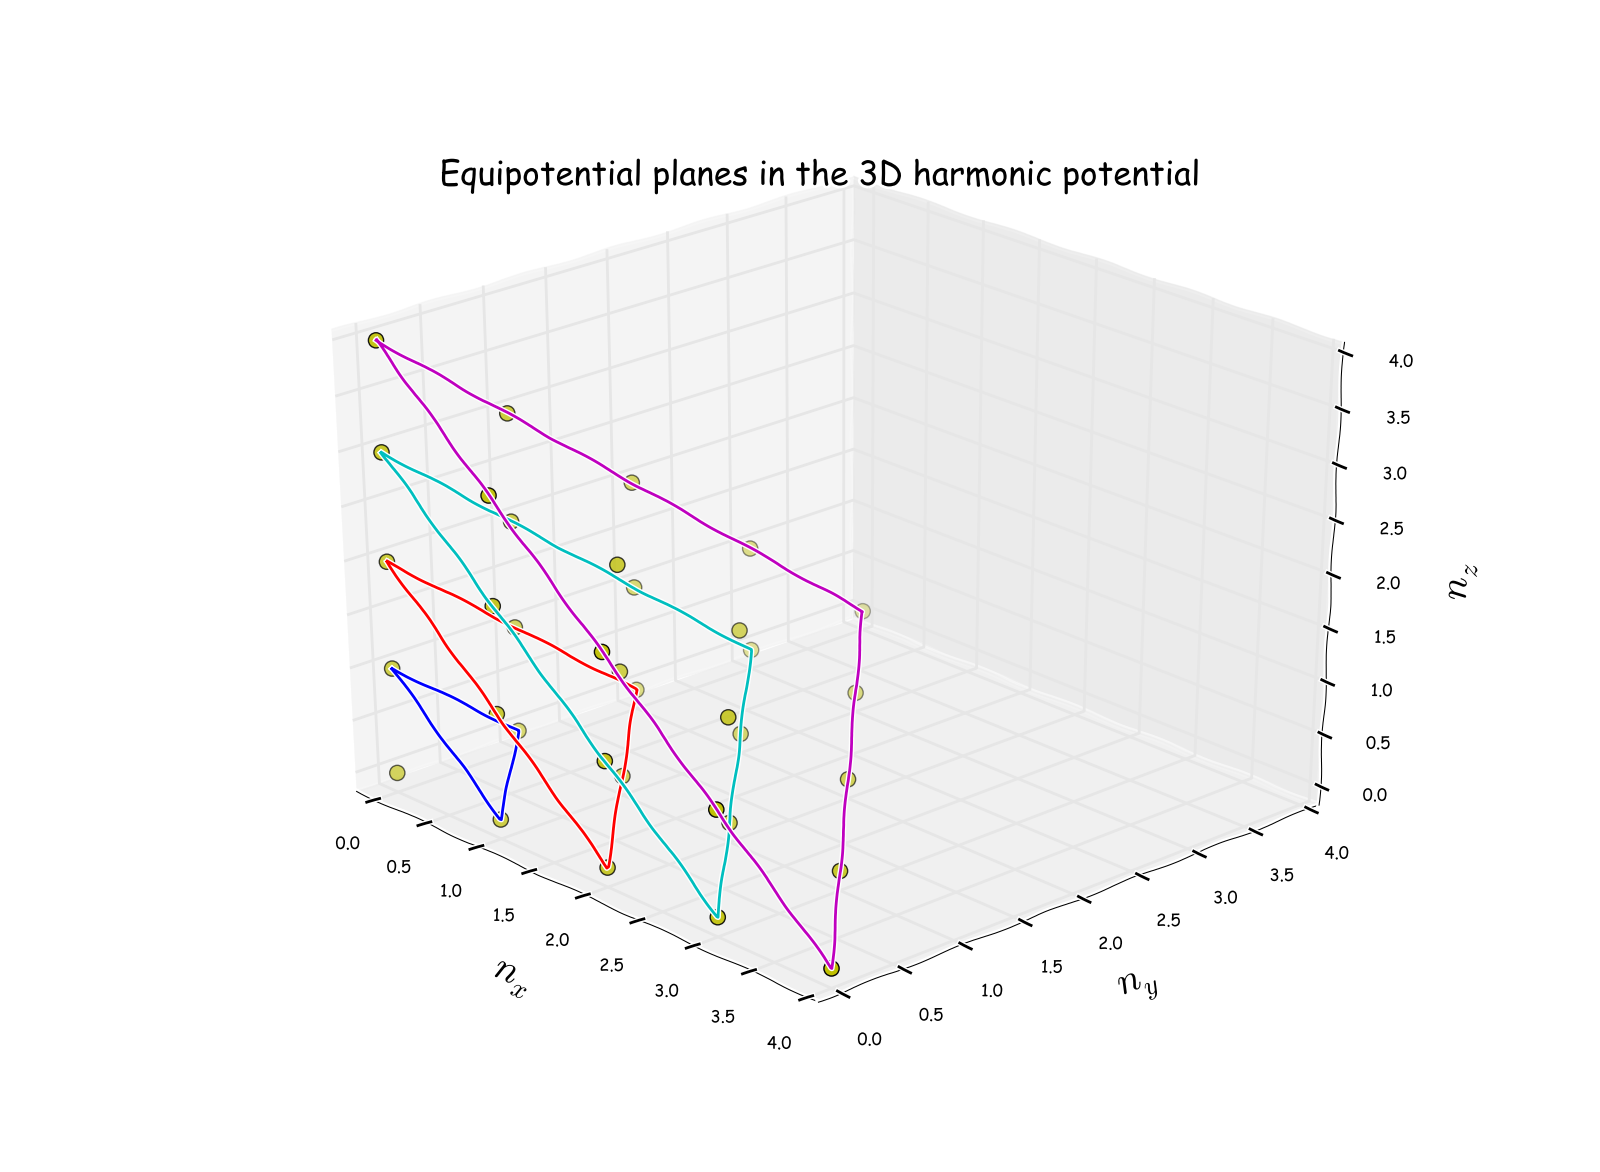
\includegraphics[width=0.7\linewidth]{eqpt3D}
	\caption{Did you know there's a context manager for matplotlib that lets you create plots that look like the webcomic xkcd? Well now you do! \cite{xkcd,mpl}}
	\label{fig:1}
\end{figure}

\section{References}
\label{sec:4}
First of all cross referencing! If one wants to refer to the image in this document there are two options -- \verb:\ref{label}:, and \verb:\cref{label}:. The first is a built in \LaTeX\ command, it works fine but is a bit clunky as it requires you to provide your own reference descriptor. To reference the image above, for example, one writes \verb;fig.~\ref{fig:1}; which typesets fig.~\ref{fig:1}. On the other hand one can use the cleveref package, which automatically identifies the environment you're referencing and describes it appropriately. The commands \verb;\cref{fig:1};, \verb;\cref{eq:1};, and \verb;\cref{sec:1};, typeset \cref{fig:1}, \cref{eq:1}, and \cref{sec:1} respectively. These labels are also fully customisable. I recommend the cleveref package.

To cite references using BibTeX one needs to include \verb:\bibliographystyle{}: somewhere in your source file, the command \verb:\bibliography{}: where you want the reference list to be placed, and to use the \verb:\cite{}: command to place citations. The argument supplied to the \verb:\cite{}: command is the citation label or key, and is the text found on the first line of the bib entry. For example in \emph{example\_OTB.bib} you will find the entry for \emph{Numerical Recipes} begins \verb:@book{NR,: so `NR' is the citation key, and the command \verb:\cite{NR}: produces the citation \cite{NR}.

Bibliography styles are given by .bst files and dictate both the citation style and the reference list style. Here I am using a modified version of the apsrev4-1 style provided by the American Physical Society for their publications (they actually even have their own `revtex' document class!). The .bib file itself is simple enough to write by hand for only a few references (or for references to websites), but many journals will let you download a bibentry directly. Referencing software such as Mendeley and EndNote can also be used to automatically create .bib files. For EndNote one needs to install a plugin which can be found at \url{http://endnote.com/downloads/style/bibtex-export}, and be sure to write a citation key into the `Label' field on the EndNote entry! Mendeley will generate a citation key for you in the format [First-author-surname][year]. For example \verb:\cite{Brown2013}: references a paper exported from Mendeley in example\_OTB.bib \cite{Brown2013}.  

The only other thing you need to know about referencing is that the document needs to be compiled twice for cross-referencing (pdflatex-pdflatex), and four times for referencing with BibTeX (pdflatex-bibtex-pdflatex-pdflatex)! Most IDEs will let you do this with a single button press. TeXworks,  Heriot-Watt's chosen LaTeX editor is not one of them.

\bibliographystyle{apsrev4-1-title}
\bibliography{example_OTB}

\end{document}
